\chapter{Propuesta}\label{chapter:proposal}

% Introducción a Deep Learning, Neural Networks: Tipos de aprendizaje, esquema de minimización.
% Explicaciones de los modelos usados: Funciones de activacion, Relu, softmax
% Explicaciones de los modelos usados: Funciones de error, categorical crossentropy
% Explicaciones de los modelos usados: LSTM y Bidireccional, CRF, CNN, ResNet, DenseLayer, GloVe, Attention
% Explicaciones de los modelos usados: Optimizadores Adam, Stocastic Gradient Descent, Diferenciacion automática

% Explicación del pipeline: Primero segmentación, luego link prediction
% Modelo de segmentación descrito a fondo
% Modelo de link prediction descrito a fondo

\section{Aprendizaje Automático}

% Hablar de problemas de regresión y de clasificación (binario y multi-class)

Existen varios problemas para los cuales es dif'icil escribir un programa de forma tradicional que pueda
resolverlo, como decir si en una imagen existe un gato o un perro, o transcribir una grabaci'on. En el caso
de que se escribiera este programa probablemente ser'ia fr'agil y poco escalable. El aprendizaje autom'atico
(\textbf{ML} por sus siglas en ingl'es \emph{Machine Learning}) constituye el estudio de t'ecnicas que puedan 
aprender de la experiencia [\cite{d2l}]. Con esto se puede automatizar el proceso de encontrar soluciones a 
dichos problemas, haciendo que sus resultados sean robustos y escalables.

Los componentes b'asicos de un problema de aprendizaje autom'atico se pueden resumir en los datos de los que 
aprender, el modelo para transformar los datos, una funci'on de p'erdida que cuantifica qu'e tan malo es el modelo 
y un algoritmo que ajuste los par'ametros del modelo para minimizar la p'erdida.

Una manera de observar la complejidad de estos modelos ser'ia la cantidad de capas de procesamiento que lo integran.
En los principios se empezaron utilizando modelos de una sola capa para realizar las tareas, m'as tarde estos modelos
fueron ganando en complejidad al superponerle otras dando paso al aprendizaje profundo.
La superposici'on se refiere
a la composici'on de funciones $f_i$ y $f_{i+1}$ de tal forma que la imagen de $f_i$ sea compatible con el dominio de 
$f_{i+1}$ entonces se obtiene $f_{i+2}(x) = f_{i+1}(f_i(x))$, al aplicar este esquema se pueden agregar m'ultiples
capas y profundizar $f$ tanto como se desee.

Matem'aticamente un modelo constituye una función $\hat{y} = f_{\theta}(x)$ a la cual se 
le pasan representaciones de las entradas orginales $x$ y devuelve una salida $\hat{y}$. Esta función $f$ se encuentra
parametrizada por el vector $\theta$ el cual constituyen los par'ametros en los que el modelo se basa para realizar sus
c'alculos. La función de p'erdida se puede definir como $e(y, \hat{y})$. El objetivo final del algoritmo de ajuste 
se define como encontrar $\theta$ tal que:

\begin{equation}
	\arg \min_{\theta} e(Y, f_{\theta}(X))
\end{equation}

% \subsection{Representaci'on de datos}

% La representación de los datos de entrada constituye una parte importante en modelar un problema. Esta 
% es la encargada de presentar datos abstractos, como im'agenes, p'arrafos, sonidos, en formas tratables
% por los algoritmos. Generalmente se buscan configuraciones que recojan la mayor cantidad de información 
% de la entrada relevante al problema. 

% En NLP la representación suele estar dada por caracter'isticas morfol'ogicas
% de las palabras, la relaciones de posición entre estas. Atributos como tamaño de palabra, 
% ..., extraen información estructural de la palabra.
% Word Embedding consiste en t'ecnicas de representación de palabras como vectores reales que codifiquen atributos
% relevantes para la tarea en cuesti'on.
% La codificación de información sem'antica es una tarea m'as desafiante. Para esto se existen varios modelos 
% como \textbf{word2vec} [TODO ref], \textbf{GloVe} (TODO Poner que signica las siglas y Referencia), \textbf{BERT}
% (TODO Poner que signica las siglas y Referencia). En \textbf{word2vec} modelan ... (TODO continuar), \textbf{GloVe}
% sigue el enfoque de ... (TODO continuar). \textbf{BERT} se basa en ... (TODO continuar, poner las variantes RoBERTa, etc).

% \subsection{Selecci'on de Modelo}

% Este proceso consiste en seleccionar la funci'on $f$ que procese los datos. Entre posibles candidatos
% se encuentran una gran variedad de funciones las cuales presentan diferentes caracteristicas que las hacen explotar
% de manera eficiente la representación y relaciones encontrados en los datos.


\subsection{Arquitecturas}

En aprendizaje profundo existen una gran cantidad de arquitecturas que se pueden utilizar para formar el modelo 
final.

\subsubsection{Capas densas}

El perceptron consiste es una transformaci'on lineal del vector de datos $\textbf{x}$ con un bias $b$ y 
luego aplicar una transformaci'on no lineal $g$, conocida como funci'on de activación, 
para la obtenci'on del resultado.

\begin{equation}
	f(\textbf{x}) = g(\textbf{\w}\textbf{x} + b)
\end{equation}\label{eq:perceptron}

El perceptron constituye la unidad b'asica de las capas densas, ya que estas consisten en la aplicaci'on
de este modelo varias veces sobre la misma entrada $\textbf{x}$ produciendo vectores de la dimensión $k$ 
deseada como salida final. Los par'ametros se codifican en la matriz $W$ y sus bias en el vactor $b$.

\begin{equation}
	f(\textbf{x}) = g(\textbf{Wx} + \textbf{b})
\end{equation}\label{eq:dense}

Para las funciones de activación existen varias elecciones. Una de estas es la función sigmoide. 
Esta devuelve un valor entre 0 y 1, es usada en tareas de regresión log'istica. 
Se puede interpretar como el nivel de activación de la neurona.

\begin{equation}
	sigm(x) = \frac{1}{1-e^{-x}}
\end{equation}\label{eq:sigmoide}

Rectified Linear Unit es definida como la parte positiva del argumento. 

\begin{equation}
	relu(x) = \max(0, x)
\end{equation}\label{eq:relu}

La funci'on de activación softmax es diferente a las anteriores en el sentido que necesita
el vector salida de la capa densa para ser computada. Esta función convierte las $q$ salidas
de una capa densa en una distribución de probabilidad.

\begin{equation}
	softmax_k(\textbf{x}) = \frac{e^(x_k)}{\sum_{i=1}^q x_i}
\end{equation}\label{eq:softmax}

\subsubsection{Redes Neuronales Convolucionales}

Las redes neuronales convolucionales (CNN por sus siglas en ingl'es) son un tipo de redes usadas
principalmente en tratar datos en los que su estructura espacial es relevante, por ejemplo
en datos bidimensionales como im'agenes y en unidimensionales como sonido y texto.
Estas redes aplican de una función de kernel sobre los datos, $f * g$ donde $f$ son los
datos, $g$ es el kernel o filtro y $*$ es el operador de convolución. La funci'on $g$ se puede 
aprender en el proceso o tambi'en puede ser una funci'on de agrupaci'on predefinida.   

Un ejemplo bidimensional de una función de kernel constituye el siguiente caso:

TODO PONER UNA FOTO DE CONVOLUCION DE KERNEL

En este se observa c'omo una nueva representación es computada al correr el kernel por la matriz de datos. Este
corrimiento se puede realizar de diferentes formas, por ejemplo se puede mover de dos en dos en vez de uno en uno, este
par'ametro se le conoce como tamanno de paso (\emph{stride} en ingl'es). Es posible adem'as preservar las dimensiones
iniciales de los datos al aplicarle un aumento de los datos en los bordes de tal forma que el resultado sea de la misma
dimensión, este aumento es generalmente rellenando con 0 los espacios convenientemente.

TODO PONER UNA FOTO DE CONVOLUCION DE KERNEL CON PADDING Y STRIDE DIFERENTE

Existen varias funciones de agrupaci'on usadas. Entre estas se encuentran las de agrupaci'on m'axima, de 
agrupaci'on media. Como sus nombres indican, la de agrupaci'on m'axima devuelve el valor m'aximo de los encontrados
en la ventana del kernel, la de media calcula el promedio de estos valores. Estas capas tienen la capacidad de obtener
información resumida sobre los datos.

\subsubsection{Redes Residuales}

Al crear modelos de aprendizaje profundo se tienen un conjunto de par'ametros, las posibles combinaciones 
de estos forman un espacio de funciones $F$ al cual pertenencen todas las posibles instancias del modelo.
Agregar nuevas capas aumenta la complejidad de este, pero no hay garant'ia de que el viejo espacio 
de funciones $F$ sea subconjunto del nuevo espacio $F'$, lo que implica que el nuevo modelo no es necesariamente
estrictamente superior al antiguo. Este problema es la raz'on de la aparici'on de las Redes Residuales. 
Una red residual est'a formada por 
uno o varios bloques residuales, en los que a la salida de cada bloque residual le es sumada la entrada de 
este mediante una conexi'on residual.
El objetivo de realizar tal operaci'on es que es posible hacer la contribuci'on del bloque 0 obteniendo as'i
un modelo equivalente a uno sin el bloque, garantizando la condici'on de subconjunto $F \subset F'$, adem'as 
dicho bloque no pierde poder expresivo dado que en caso de que su aporte sea considerable al resultado final, 
se tendr'ia que aprender solamente la funci'on $f(x) - x$ donde $x$ es la entrada del bloque para mitigar el 
efecto de la conexión residual y $f$ es la funci'on aprendida por el bloque sin la conexi'on residual.

TODO FOTO DE RESNET. d2l pag 289

\subsubsection{Redes Neuronales Recurrentes}

% Definicion de RNN, LSTM, Bidireccional, Ventajas de RNN en secuencias
Las redes neuronales recurrentes (\textbf{RNN} por sus siglas en inglés \emph{Recurrent Neural Networks}) son
un tipo especial de arquitectura especializada en el trabajo con datos secuenciales. Este tipo de arquitecturas
presentan variables en las que se almacenan información pasada que es usada para el computo de la salida. El 
problema se puede modelar mediante probabilidades mediante la estimaci'on de $P(x_t | x_{t-1}, \dots x_{1})$,
donde existen dos variantes principales, se fija un tamanno de ventana en el tiempo $\alpha$ dando como resultado
$P(x_t | x_{t-1}, \dots, x_{t-\alpha})$ a este tipo de modelos se les conoce como autoregresivos. Otra estrategia
consiste en guardar un contexto de observaciones pasadas $h_t$ y con este realizar la estimaci'on $P(x_t | h_t)$,
el contexto se actualiza en cada paso mediante una funci'on $h_t = g(h_{t-1}, x_{t-1})$, a estos se les nombra
modelos autorregresivos latentes. 

Estos modelos presentan problemas de gradientes ya que estas pueden volverse extremadamente grandes o desaparecer.
Para esto se han creado arquitecturas que disminuyen estos problemas. Una de estas arquitecturas es las memorias
de corto largo plazo (\textbf{LSTM} for sus siglas en ingl'es \emph{Long Short Term Memory}) [\cite{TODO lstm}].
Este modelo guarda un contexto del procesamiento y est'a constitu'ido por varias compuertas que regulan las 
actualizaciones de los estados internos. \textbf{LSTM} posee dos variables de estado, la memoria $C$ y el estado 
oculto $H$. Entre sus compuertas se encuentran la compuerta de olvido, esta regula cuanto de la memoria permanece
en el proximo paso, la compuerta de entrada ajusta la cantidad de información nueva que estrar'a, la compuerta 
de salida maneja el calculo del pr'oximo estado oculto.

TODO FOTO DE LSTM d2l pag 357

El m'etodo de aprendizaje de las \textbf{RNN} solamente observa los elementos anteriores de la secuencia, aunque existen
tareas en las que observando los elementos posteriores brinda m'as contexto e información a la tarea sin que interfiera
en el proceso de inferencia. El modelo bidireccional presenta una alternativa para tratar estas tareas, este modelo
consiste en adem'as de hacer la corrida de inicio a final de la secuencia, se realiza un desde al final hasta el  
inicio de esta, estas corridas van generando dos estados ocultos $\overrightarrow{H}_{i}$ y $\overleftarrow{H}_{i}$
que luego son mezclados para obtener el contexto final $H_i$.

TODO FOTO DE BIDIRECTIONAL LSTM d2l pag 367

\subsubsection{Atención}

% Definicion, qué hace, uso en secuencias
La atenci'on es una t'ecnica en la cual se hace una selecci'on ponderada de atributos en un contexto espec'ifico. 
Este mecanismo presenta dos partes, una consulta $q$ y una collecci'on de pares llave-valor $(k_i, v_i)$, la 
consulta representa el contexto en donde se quiere aplicar la atenci'on y las llaves $k_i$ son elementos que 
relacionan la consulta a los valores $v_i$. El proceso de calcular el resultado consiste en primero calcular 
el vector compatibilidad $e$ entre las llaves y la consulta mediante la función $f$, este vector es luego 
modificado por una función $g$ que distribuye los valores obteniendo el vector atenci'on $a$, finalmente 
este vector es utilizado para calcular el resultado final al aplicarle la función $o = z(a, V)$.

\begin{equation}
	\begin{align}
		e = f(q, K) \\
		a = g(e) \\ 
		o = z(a, V)
	\end{align}
\end{equation}

En dependencia de c'omo se seleccionen las funciones $f$, $g$ y $z$ se pueden obtener distintos tipos de atenci'on.
Una configuraci'on simple consiste en ser $f$ definida como el producto punto de la consulta con la llave,
$g$ softmax y $z$ la suma ponderada de $v_i$ con los valores de atención. 

\subsubsection{Campo Aleatorio Condicional}

% Definicion de CRF, qué modela, Ventajas de CRF en secuencias, mirar relacion con Hidden Markov Models

El campo aleatorio condicional (\textbr{CRF} por sus siglas en ingl'es \emph{Conditional Random Field}) es un 
tipo de modelo gr'afico probabil'istico con el objetivo de modelar eficientemente el trabajo con secuencias 
modelando conjuntamente la probabilidad de las etiquetas de las secuencias dada sus observaciones [\cite{lafferty2001conditional}].
En trabajos de secuencias la forma m'as simple que toma el grafo consiste en una cadena de las variables representando
las etiquetas de las secuencias $Y$ conectadas de la forma $(Y_i, Y_{i+1})$ y las variables observadas $X$ conectadas
a las variables $Y$ [\cite{wallach2004conditional}].

El objetivo de \textbf{CRF} es calcular la secuencia $Y^*$ tal que:

\begin{equation}
	\arg \max_Y P(Y | X)
\end{equation}\label{eq:crf}

En este \ref{eq:crf} se observa que devuelve la secuencia m'as probable dado las variables observadas o atributos $X$,
por lo que esta capa es usada al final para problemas de clasificaci'on de secuencias.

\subsection{Evaluaci'on del modelo}

En \textbf{ML} los modelos necesitan maneras de expresar qué tan buenos son 
en las tareas encomendadas. Para esto se crean funciones que evalúan los resultados obtenidos
por dichos modelos, estas funciones se les da el nombre de métricas. Existen diferentes tipos de
métricas para tratar con diferentes tipos de problemas. En aprendizaje supervisado una métrica se
define como una función $m_s(Y, \hat{Y})$ donde $Y$ son las predicciones verdaderas y $\hat{Y}$ son las predicciones
hechas por el modelo. En algoritmos de aprendizaje no supervisado como K-Means, K-NN son usadas funciones $m_{ns}(\hat{Y})$
donde $\hat{Y}$ son las predicciones finales. En comparación con su versión supervisada estas funciones no tiene acceso
a las predicciones verdaderas del problema.

\subsubsection{Regresión}

En problemas de regresión se emplean comúnmente
métricas como error medio cuadrático (MSE por sus siglas en inglés \emph{Mean Squared Error}), 
raíz de MSE (RMSE por sus siglas en inglés \emph{Root Mean Squared Error}),
error medio absoluto (MAE por sus siglas en inglés \emph{Mean Absolute Error}) y error absoluto promedio porcentual 
(MAPE por sus siglas en inglés \emph{Mean Absolute Percentage Error}) [\cite{botchkarev2019new}].

\begin{figure}
	\begin{equation}\label{metric:MSE}
		mse(Y, \hat{Y}) = \frac{1}{N} \sum^{N}_{i=1} (Y_i - \hat{Y}_i)^2
	\end{equation}
	\caption{MSE}
\end{figure}

\begin{figure}
	\begin{equation}\label{metric:RMSE}
		rmse(Y, \hat{Y}) = \sqrt{mse(Y, \hat{Y})}
	\end{equation}
	\caption{RMSE}
\end{figure}

\begin{figure}
	\begin{equation}\label{metric:MAE}
		mae(Y, \hat{Y}) = \frac{1}{N} \sum^{N}_{i=1} |Y_i - \hat{Y}_i|
	\end{equation}
	\caption{MAE}
\end{figure}

\begin{figure}
	\begin{equation}\label{metric:MAPE}
		mape(Y, \hat{Y}) = \frac{1}{N} \sum^{N}_{i=1} |\frac{Y_i - \hat{Y}_i}{Y_i}|
	\end{equation}
	\caption{MAPE}
\end{figure}

\subsubsection{Clasificación}

En problemas de clasificación son empleadas otras medidas que toman en cuenta la naturaleza discreta del problema. 
Medidas como precisión, recobrado, certeza (accuracy en inglés) y F1 son utilizadas principalmente en la 
evaluación de los resultados, mientras que como función de error se usa entropía cruzada com'unmente 
(\emph{cross entropy} en inglés) [\cite{grandini2020metrics}].

La matriz de confusión es una via de representar los resultados de dos clasificadores. Esta matriz en $M_{ij}$ 
indica la cantidad de elementos que clasificó como clase $i$ el primer clasificador y
como clase $j$ el segundo clasificador. En su uso práctico
un clasificador son las etiquetas verdaderas mientras que el otro es el clasiificador que se está evaluando. 
En problemas de la clasificación binaria, donde se busca saber si existe pertenencia o no de un elemento a una clase,
se pueden observar los siguientes casos.

\begin{itemize}
	\item Verdaderos Positivos (VP): Elementos clasificados correctamente que pertenecen a la clase.
	\item Verdaderos Negativos (VN): Elementos clasificados correctamente que no pertenecen a la clase.
	\item Falsos Positivos (FP): Elementos clasificados incorrectamente que pertenecen a la clase.
	\item Falsos Negativos (FN): Elementos clasificados incorrectamente que no pertenecen a la clase.
\end{itemize}

TODO FOTO DE MATRIZ DE CONFUSION BINARIA

La precisión es la medida que indica la probabilidad de que la clasificación de una clase sea correcta. Esto 
se puede observar como la proporción de los elementos correctamente clasificados sobre el total de 
elementos clasificados:

\begin{equation}
	prec_i = \frac{VP}{VP + FP}
\end{equation}

En problemas de clasificación múltiple surge la versión macro de esta medida calculada como la media de todas
las precisiones de las clases existentes:

\begin{equation}
	prec_{macro} = \sum^K_{i=1} \frac{prec_i}{K}
\end{equation}

El recobrado es la medida que indica la probabilidad de que se clasifique correctamente un elemento de la clase
del total existente. Esto se puede observar como la proporción de los elementos correctamente clasificados sobre el 
total de elementos que pertenecen a la clase:

\begin{equation}
	rec_i = \frac{VP}{VP + FN}
\end{equation}

En problemas de clasificación múltiple surge la versión macro de esta medida calculada como la media de todos
los recobrados de las clases existentes:

\begin{equation}
	rec_{macro} = \sum^K_{i=1} \frac{rec_i}{K}
\end{equation}

La medida F1 es la media armónica de la precisión y el recobrado. En esta la contribución de la precisión y el
recobrado al resultado final es el mismo, aunque es posible buscar variaciones de acuerdo a al problema a tratar:

\begin{equation}
	f1_i = 2 (\frac{prec_i * rec_i}{prec_i + rec_i})
\end{equation}

En problemas de clasificación múltiple surge la versión macro de esta medida calculada la propia medida F1 pero
utilizando la precisión y recobrado macro del problema:

\begin{equation}
	f1_{macro} = 2 (\frac{prec_{macro} * rec_{macro}}{prec_{macro} + rec_{macro}})
\end{equation}

La entropía cruzada se encarga de evaluar qué tan diferentes son dos funciones de distribución $p$ y $q$, por lo que
pequeños valores de esta indican mayor similitud. En su versión discreta se formula:

\begin{equation}
	H(p, q) = - \sum_{x \in D} p(x) \log q(x)
\end{equation}

\subsubsection{Curvas de aprendizaje}

Es necesario adem'as de evaluar el resultado final del modelo, evaluar el proceso de entrenamiento. En esta etapa 
se pueden diagnosticar varias deficiencias en este proceso. Para un correcto diagn'ostico se divide el conjunto de 
datos en tres partes:

\begin{itemize}
	\item \textbf{entrenamiento}: Utilizada para el entrenamiento del modelo.
	\item \textbf{validaci'on}: Utilizada para evaluar el desempenno del modelo en entrenamiento.
	\item \textbf{prueba}: Utilizada para evaluar el resultado final.
\end{itemize}

Las curvas de aprendizaje constituye la principal herramienta para evaluar el proceso de aprendizaje.
Estas est'an formadas por las mediciones de m'etricas a lo largo del entrenamiento calculadas a partir de 
los conjuntos de validaci'on y entrenamiento. La linea correspondiente al conjunto de entrenamiento cuantifica 
el aprendizaje del modelo o también el error de entrenamiento y la correspondiente al de validación la 
generalizaci'on o el error de generalizaci'on. Existen tres comportamientos escenciales:

\begin{itemize}
	\item Bajo ajuste (\emph{underfitting} en ingl'es)
	\item Sobreajuste (\emph{overfitting} en ingl'es)
	\item Buen ajuste
\end{itemize}

El bajo ajuste ocurre cuando el modelo no es capaz de aprender del conjunto de datos o cuando este a'un puede aprender 
m'as. Las curvas de aprendizaje en estos casos se caracterizan por ser una linea plana o valores ruidosos con alta p'erdida.

TODO FOTO de LO DICHO ANTERIOR. Guiarse por el libro [brownlee2018better]

Entre las formas m'as sencillas de combatir el bajo ajuste de los modelos consiste en complejizar el modelo, al annadir
capas o aumentar las dimensiones se este aumenta la expresividad de este y por lo tanto su ajuste. Si este m'etodo 
no funciona es posible considerar un cambio de arquitectura hacia una que pueda extraer m'as información de la 
estructura de los datos. 

El sobreajuste es el fen'omeno en el que el modelo se aprende los datos de entrenamiento extremadamente bien, incluso
el ruido en estos datos, esto trae consigo que falla en generalizar el problema para nuevas entradas. Las curvas 
caracter'isticas de este fen'omeno presentan una divergencia en los errores de entrenamiento y validación a medida
que se entrena el modelo, mientras que la de entrenamiento mejora la de validación tiende a empeorar. 

TODO FOTO de OVERFITTING. Guiarse por el libro [brownlee2018better]

Existen varios m'etodos para combatir el sobreajuste, uno sencillo es simplificar el modelo quit'andole capas 
o disminuyendo sus dimensiones. Adem'as de esto existen regularizaciones que se pueden aplicar para evitar que 
las capas dependan exclusivamente de pocos atributos, entre esta familia los m'as usados son la regularizaci'on
L1 y L2 las cuales se definen como la suma del valor absoluto de los atributos y la suma del cuadrado de sus 
atributos respectivamente. Otra medida para prevenir el sobreajuste es el agrego de capas de abandono 
(\emph{dropout} en ingl'es), estas capas desactivan neuronas de la arquitectura y obligando a 
estas a ser robustas y depender del comportamiento de la población, en lugar de la actividad de otras unidades 
específicas [\cite{baldi2013dropout}]. La terminaci'on temprana (\emph{early stopping} en ingl'es) del entrenamiento
se utiliza para parar este en el momento en que el error de generalizaci'on comienza a subir, impidiendo as'i que 
se sobreentrene el modelo.

Finalmente un buen ajuste es el resultado que se alcanza cuando tanto la curva de validación como de entrenamiento
presentan valores pequennos y similares, consecuentes con una correcto aprendizaje y generalizaci'on.

TODO FOTO de Good Fit. Guiarse por el libro [brownlee2018better]

Otro problema observable a partir del an'alisis de las curvas de aprendizaje constituye la detecci'on de conjuntos
de datos no representativos. Un conjunto de datos no representativo es uno que puede no 
capturar las características estadísticas relativas a otro conjunto de datos extraído del mismo dominio.
Esto puede pasar que los conjuntos de entrenamiento o de validación. En caso del conjunto de entrenamiento
se puede identificar si la p'erdida en el conjunto de entrnamiento conlleva a una ganancia en el conjunto de 
validación y viceversa quedando al final con una separaci'on entre ambos valores. En el caso del conjunto de 
validación se presenta como una curva ruidosa, también se puede dar el caso de que el conjunto  de validación
sea m'as f'acil de predecir que el de entrenamiento, en este caso se observa como la curva de validación permanece
siempre por debajo de la de entrenamiento.

TODO FOTO de Unrepresentative Train Data, Unrepresentative Dev Data (Noise, Easier than train). Guiarse por el libro [brownlee2018better]

Para combatir estos problemas se puede aumentar la cantidad de elementos en los conjuntos de entrenamiento o 
validación en dependencia de donde ocurra.

\subsection{Aumento de datos}

El aumento de datos consiste en acciones para aumentar la diversidad de un conjunto de datos sin recolectar
nuevos datos expl'icitamente [\cite{feng2021data}]. En datos continuos, como im'agenes o valores num'ericos el 
aumento de datos puede ser realizado al annadirle perturbaciones a entradas existentes, en caso de las im'agenes 
t'ecnicas como el volteado (\emph{flipping}) o recortado (\emph{cropping}) son usadas. Los textos son un tipo 
de datos discreto y por lo tanto las t'ecnicas anteriores no pueden ser aplicadas directamente. Para \textbf{NLP}
se han estudiado diversas t'ecnicas para el aumento de datos, una de estas consiste en el cambio del 'arbol de 
dependencia de la oración mediante operaciones de intercambio y borrado de nodos, también se han utilizado 
gaceteras para el intercambio de palabras por sin'onimos, la traducción de textos hacia un lenguaje y luego 
de vuelta al lenguaje origen es otro ejemplo. 

\subsection{Aprendizaje Conjunto}

El aprendizaje conjunto (\emph{ensemble learning} en inglés) constituyen t'ecnicas encaminadas al aprovechamiento
de soluciones encontradas por diferentes modelos combin'andolas y mejor'andolas para encontrar una mejor soluci'on 
al problema. Estos m'etodos son efectivos en la reducción de la varianza y el bias de los resultados obteniendo as'i
mejores modelos [\cite{dietterich2002ensemble}] 

Dado que en TODO 

\subsection{M'etodos de optimizaci'on}

Optimizaci'on, encontrar la solucion exacta es un problema dificil, se usan metodos para buscar soluciones aproximadas.
Descenso por gradiente Algoritmo general, Optimizadores (Adams, Stocastic Gradient Descent, Exponential Decay)

El objetivo de \textbf{ML} es encontrar los extremos de una función de costo, este proceso es una tarea 
desafiante ya que la gran mayor'ia de estas funciones no son convexas y por lo tanto no existe un algoritmo
que asegure la convergencia hacia un extremo global. Para resolver este problema exiten m'ultiples heur'isticas,
la m'as usasda es el descenso por gradiente, este algoritmo contiene m'ultiples variaciones. La idea b'asica consiste 
en el c'alculo del vector gradiente de la funci'on de error $e$ con respecto a los par'ametros del modelo $x$ y una vez se 
tiene dicho vector se evalua en la asignaci'on actual de los par'ametros $x_i$ y se realiza un corrimiento de este punto 
en contra del gradiente para disminuir el error.

\begin{equation}
	x_{i+1} = x_i - \alpha \nabla f(x_i)
\end{equation}\label{eq:gradien_descent}

En la ecuaci'on anterior $\alpha$ se le conoce como tasa de aprendizaje (\emph{learning rate} en ingl'es).

Variantes de este algoritmo eficientes para el proceso de entrenamiento de modelos de \textbf{ML} han sido 
creadas. Una de estas variantes es el descenso por gradiente estoc'astico

\subsection{Procesamiento de Secuencias}

Modelos sequence to sequence


\section{Modelo Propuesto}

El modelo propuesto se divide en dos secciones. En la primera sección se realiza la segmentación y clasificación de 
las UDAs como tareas conjuntas. En la segunda sección se predicen los enlaces y sus clasificaciones, tomando
como tareas auxiliares la clasificación de las UDAs. En dependencia de los resultados obtenidos, la clasificación final de 
las UDAs se escoge de la mejor sección (TODO IMPLEMENTAR ESTO, O NO). 
Dada la heterogeniedad de las conjuntos de datos disponibles en EA estos modelos poseen un m'inimo de 
atributos hechos a mano, esto permite que el modelo por s'i solo aprenda la mejor representación para el
esquema de anotaci'on con que se entrene. 

\subsection{Segmentación y clasificacón de UDAs}

Esta primera parte se modeló como un problema secuencia a secuencia cuyo objetivo es convertir la secuencias de 
tokens en secuencias de etiquetas BIOES. Además de las anotaciones BIOES se agrega información sobre el 
tipo de UDA al que pertenece el segmento.

\subsubsection{Modelo}

Sea $D$ un documento entrada, este es separado en una secuencia de $n$ tokens $D_i$ donde $n$ es la mayor longitud encontrada
en los documentos del conjunto de datos (si la cantidad de tokens es menor que $n$ entonces $D_i$ es completado con un token especial de enmascarado). 
A cada token se le es asignado
su representación vectorial \textbf{GloVe} de dimensión $g$ dando como resultado $G_{ij} \in \mathbb{R}^{n \times g}$.
Esta representación inicial presenta información semántica de las palabras además que conserva las relaciones 
espaciales entre ellas. 

Para la representación de información morfológica de la palabra se construyen dos
codificadores que procesan los caracteres de cada token y devuelven una representación vectorial de estos.
A cada caracter se le es asignado un vector que será entrenado convirtiendo un token en un vector de dimensión
$q \times c$ donde $q$ es el tamaño máximo de palabra en el conjunto de datos y $c$ es la dimensión del vector
asignado a cada caracter.
Uno de estos modelos está basado en \textbf{CNN}, este modelo entrena una representación de caracteres de dimensión
$cd$ representando un token como un vector de dimensión $q \times cd$. Se conforma por una capa de convolución unidimensional
con $f$ filtros y un kernel de tamaño $k$ seguida por un \textbf{Max Pool Layer} que convierte la secuencia en un vector
de dimensión $1 \times f$ que luego este vector es concatenado a la representación del token a que pertenece.
Otro modelo utilizado para calcular una representación morfológica se encuentra basado en \textbf{RNN}. Se usó
un modelo LSTM bidireccional con dimensión $l$ para calcular la representación del token, para las dimensiones de los caracteres se
utilizan vectores de tamaño $l$, el resultado final constituye la concatenación de la corrida hacia adelante y
hacia atrás formando una representación de dimensión $1 \times 2l$ del token. Este vector es concatenado a la representación
del token correspondiente.

Otro atributo usado en la representación de los tokens constituyen las etiquetas de Partes de la Oración de estos.
El conjunto de etiquetas elegido es un conjunto universal [TODO \cite{Referencia a la def}] aplicable a cualquier idioma.
De estas etiquetas se les extraen la codificación one-hot y esta es transformada por una capa densa con $p$ neuronas
y función de activación \textbf{relu}, el resultado es concatenado a la representación del token correspondiente.

Del proceso de vectorización sale un vector con dimensión $n \times t$ donde $t$ es la dimensión final de la representación
de los tokens. Este vector es modificado por una capa \textbf{LSTM} bidireccional de dimensión $m$, a esta salida se le 
añade una conexión residual al ajustarle la dimensión con una capa densa. Luego la secuencia es procesada por una 
capa densa de dimensión $k$ produciendo una representación final de dimensión $q \times k$.
Finalmente se utiliza una capa \textbf{CRF}
para la clasificación final de la secuencia en las etiquetas finales. El resultado final constituye un vector
de dimensión $q$ que representa las clasificaciones inferidas por el modelo.

\begin{figure}[h!]
	\begin{center}
		\begin{center}
			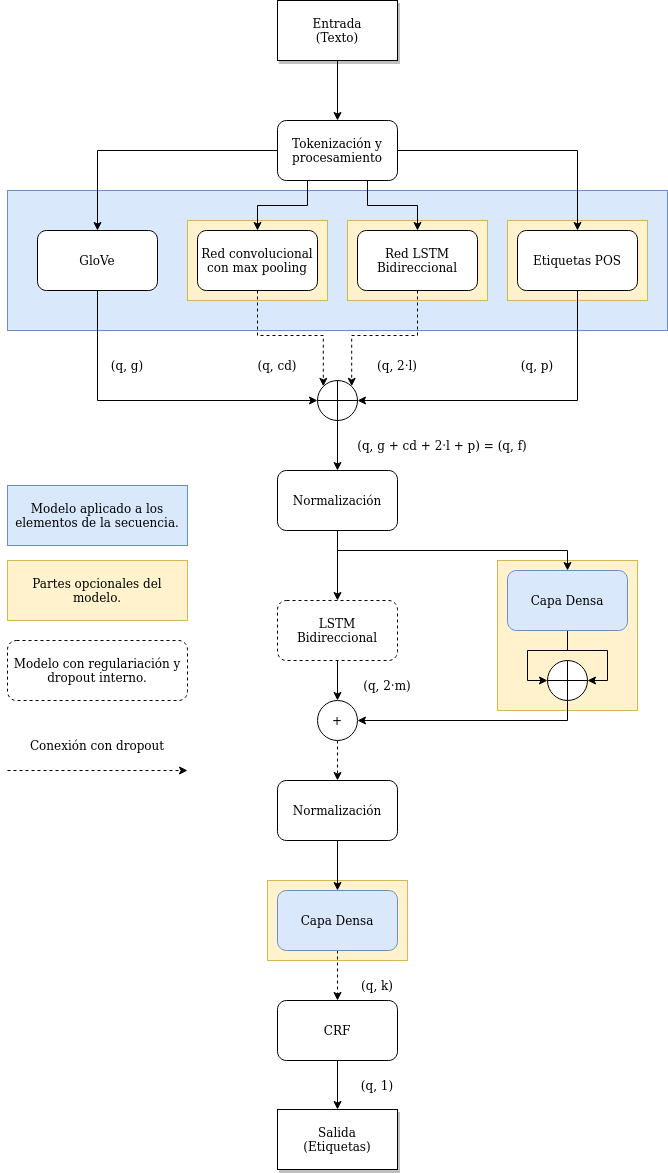
\includegraphics[scale=.3]{Graphics/Modelo_Segmenter_UDA.png}
            % \includesvg[options]{Graphics/Modelo Segmenter UDA.svg}
        \end{center}
	    \caption{Segmentador UDAs}\label{fig:seg_uda}
	\end{center}
\end{figure}

Debido a la escasez de los datos se tuvieron que tomar medidas para prevenir el overfitting. Entre cada capa de 
procesamiento se añadieron capas de normalización y \emph{dropout} con un porciento de $d$\%. Además de esto se 
las capas densas y de \textbf{LSTM} se utilizaron regularizaciones L2. Como optimizador se utilizó Adam.

\subsubsection{Posporcesamiento}

La salida del modelo constituye una secuencia de etiquetas en formato BIOES. La secuencia devuelta puede que contenga
errores en la estructura BIOES, por ejemplo, secuencias no terminando en E, segmentos continuos con más de una meta-etiqueta.
Para la corrección de la estructura se propone el siguiente algoritmo, el cual se divide en dos partes. La primera
parte consiste en arreglar la estructura BIOES, para esto se mantiene una ventana de tamaño
3 sobre la secuencia y asume que la parte anterior a la posición de la ventana no presenta errores, al encontrar una
ventana inválida se necesita observar la siguiente ventana para poder decidir cómo se arregla el error ya que se
podría dar el caso de OOI OIO, en donde solamente viendo la primera ventana no se podría saber si el cambio 
correcto corresponde a sustituir I por B o por S. Una vez observado las dos ventanas se procede a realizar el 
arreglo correspondiente. Una vez se tiene la secuencia tiene la estructura BIOES correctamente anotada el problema
consiste en arreglar las meta-etiquetas, ya que una misma secuencia BIOES pudo haber sido anotada con diferentes
tipos de meta-etiquetas, en este caso se toma la etiqueta más representativa de la secuencia. Este procedimiento
devuelve una secuencia BIOES correctamente anotada.

\subsection{Predicción de enlaces}

Este modelo consiste en dados dos pares de UDA previamente extraídas, 
extraer y clasificar la relación entre ellas, como tarea auxiliar se realiza además la clasificación 
de las UDAs. Su salida consiste en una tupla conteniendo las clases de relación, tipo de UDA fuente y 
tipo de UDA objetivo respectivamente $(r \in R, s \in U, t \in U)$ donde $R$ y $U$ son los conjuntos de 
posibles relaciones y UDAs del corpus con que se entrena.

\subsubsection{Modelo}

Sea dos UDAs, $S$ y $T$, una representa la fuente de la relación, mientras que la otra representa
el objetivo. Estas secuencias son tokenizadas y se les asigna la representación GloVe de cada palabra, obteniendo
dos vectores de dimensión $u \times g$, donde $u$ es el tamaño máximo de UDAs en el conjunto de entrenamiento.
Estos vectores son modificados por una red densa compuesta por $ca$ capas con activación \textbf{relu}. 
Al finalizar este procesamiento se añade una conexión residual
a la salida. El próximo paso consiste en aplicar una capa densa de dimensión $di$ y luego un \emph{average pooling}
de tamaño $dp$, obteniendo vectores de dimensión $\frac{q}{di} \times dq$. 
Estos vectores son modificados por un \textbf{LSTM} bidireccional con $lm$ unidades. Un módulo de atención es aplicado 
sobre los vectores fuentes, 
en este actúan como consultas el promedio de los vectores objetivo y como llaves y valores los vectores fuentes,
el procedimiento simétrico es realizado para los vectores objetivos.
La salida de los procesamientos son concatenados con la distancia argumentativa obteniendo una representación 
conjunta de la relación a analizar. Esta representación conjunta es modificada por una red residual obteniendo
una representación final de dimensión $ff$ y luego sometida a los clasificadores de relación y de tipos de UDAs.

\begin{figure}[h!]
	\begin{center}
		\begin{center}
			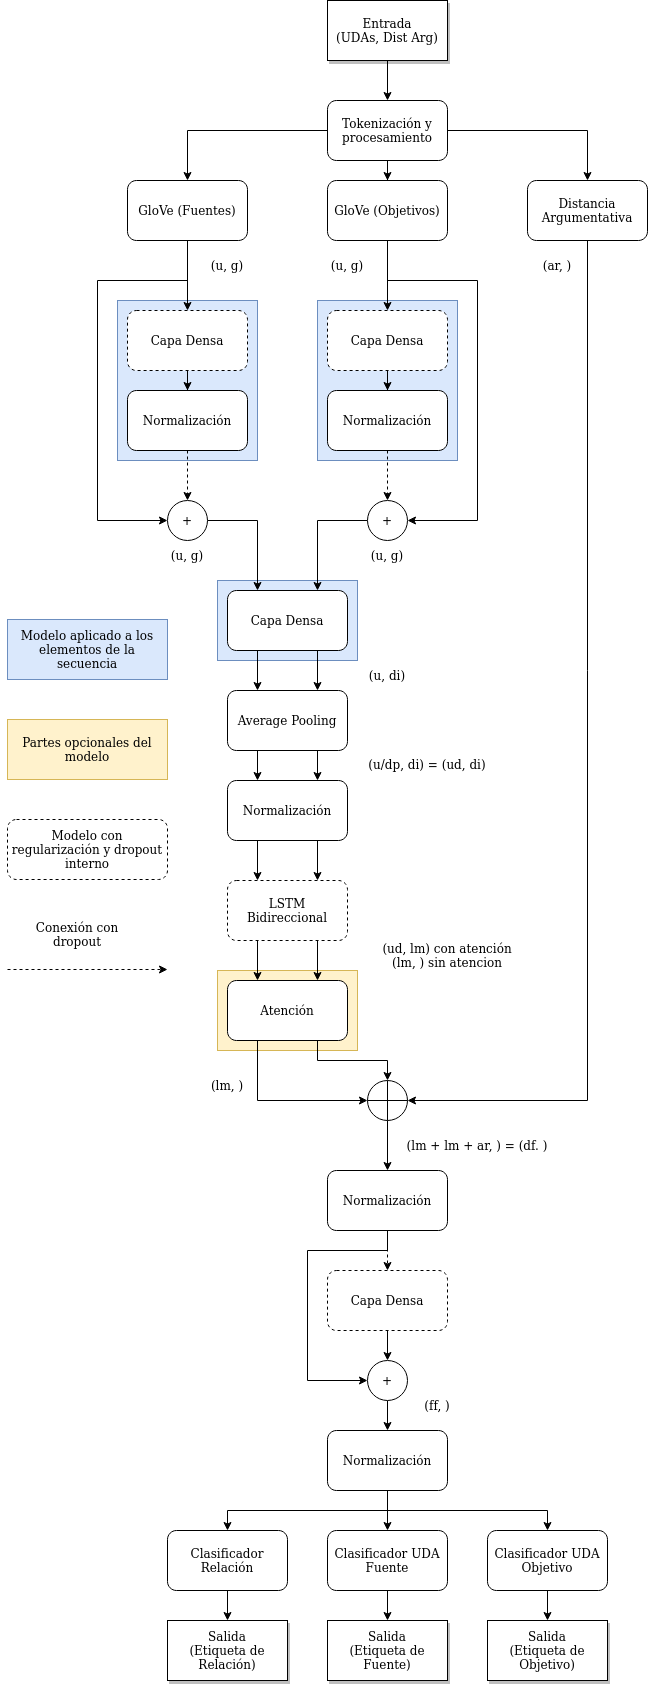
\includegraphics[scale=.3]{Graphics/Modelo_Link_Prediction.png}
            % \includesvg[options]{Graphics/Modelo Link Prediction.svg}
        \end{center}
	    \caption{Predictor de enlaces}\label{fig:link_predictor}
	\end{center}
\end{figure}

Para prevenir el overfitting se agregaron capas de normalización y de dropout entre cada proceso y se usaron regularizaciones
L2 en las capas densas y \textbf{LSTM}. Como optimizador se utilizó Adam con descenso exponencial.

